\chapter{Herramientas utilizadas}\label{Herramientas utilizadas}
%Función que crea el título de capítulo y al cual se le da el nombre deseado a través de su parámetro obligatorio. Al no tener la función el “*” se escribirá también en el título del documento las palabras “Capítulo 1: …”. Además se indica, mediante la función “\label”, la correspondiente etiqueta que lleva asociada. La etiqueta sirve para que en caso de que luego se quiera hacer referencia al capítulo se haga llamando etiqueta tal que se escribiría “La información correspondiente a dicho tema se encuentra en el capítulo \ref{Int}.”

\thispagestyle{fancy}
%Función que determina que durante este capítulo se aplique el estilo Fancy.

\fancyhead[LE]{\thechapter.Herramientas utilizadas} 
%Función que se utiliza para indicar que en las páginas impares, aparezca en el encabezado en la parte izquierda, el número del capítulo con su correspondiente nombre.
A continuación se procederá a detallar y a analizar las herramientas utilizadas para el funcionamiento de este PFG. Las herramientas de desarrollo estarán especificadas en el apartado de metodología \ref{Metodología}.
\section{React}
React es una opción muy buena para crear UI responsivas y fácilmente actualizables. Como en este proyecto se están escuchando a eventos de la red y actualizando todo constantemente, utilizar este framework es una gran opción. React nos ofrece \textit{hooks} para actualizar la interfaz del usuario. 
En los siguientes puntos del proyecto se explicará con detalle el uso de react en esta aplicación.
\section{Metamask}
Metamask es un wallet que se puede comunicar con la blockchain de ethereum que dispone de funcionalidades de firma, encriptación y desencriptación muy útiles para este proyecto. Existe como una extensión en el navegador y también tiene la capacidad de usarse desde el dispositivo móvil.
\section{OrbitDB}
Base de datos distribuida. Ha sido construida por encima de \verb|js-ipfs \cite{web:js-ipfs}| (una librería que convierte nuestro navegador en un nodo de IPFS \cite{web:ipfs}). Utiliza su sistema de peers para poder compartir datos utilizando una ruta a la que se puede acceder. Gracias a la criptografía, se pueden implementar permisos de lectura y escritura. Los datos de la base de datos se guardan en el \verb|local storage| del navegador.
El funcionamiento es totalmente nuevo a los paradigmas actuales. Principalmente por la naturaleza inmutable de IPFS \cite{web:ipfs}. La dirección hace referencia a un fichero en IPFS \cite{web:ipfs}.\\
\verb|/orbitdb/Qmd8TmZrWASypEp4Er9tgWP4kCNQnW4ncSnvjvyHQ3EVSU/database-name|\\
Esta URL, contiene las siguientes partes.
\begin{itemize}
    \item \textbf{/orbirdb/}: hace referencia a que el fichero existe en una carpeta llama orbitdb. Esto se hace por simplicidad. Todos los proyectos introducen sus datos bajo las carpetas para poder saber a quien pertenecen de un vistazo.
    \item \textbf{Qmd8TmZrWASypEp4Er9tgWP4kCNQnW4ncSnvjvyHQ3EVSU}: Esta sección es generada aleatoriamente. Principalmente para evitar conflictos. Esto genera un problema, ya que al ser aleatorio no podemos saber cual es la base de datos de nuestro peer al que queremos contactar. Este problema se solucionará más adelante en el proyecto.
    \item \textbf{database-name}: En este ultimo apartado es libre. Esto significa que como ya hemos evitado conflictos entre bases de datos, podemos aportar un nombre útil para la aplicación. En el caso de este proyecto, se utiliza la dirección de la carte del usuario. 
\end{itemize}
En esta dirección vive un archivo que solamente tiene la clave publica de orbit db. De este modo, todos los usuarios que se quieran conectar pueden leer la clave con la seguridad de que no ha sido manipulada.
\begin{figure}[h!]
    \centering
    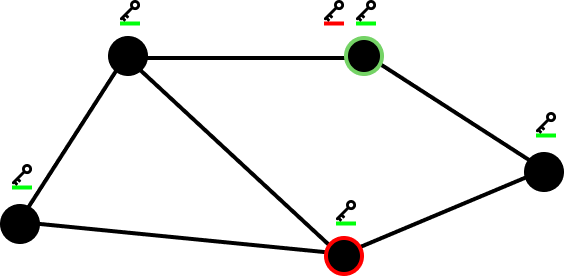
\includegraphics[width=0.7\textwidth]{Figures/Orbitdb.png}
    \caption[Diagrama básico de conexión de orbitdb]{Diagrama que ejemplifica una base de datos compartida en el que el nodo propietario es el verde.}
    \label{fg:orbit}
\end{figure}
En el siguiente escenario \ref{fg:orbit}, hay una serie de nodos escuchando al nodo con la clave publica que han podido obtener del fichero. Al mismo tiempo, todos escuchan al mismo topic que han obtenido desde el fichero.
\begin{figure}[h!]
    \centering
    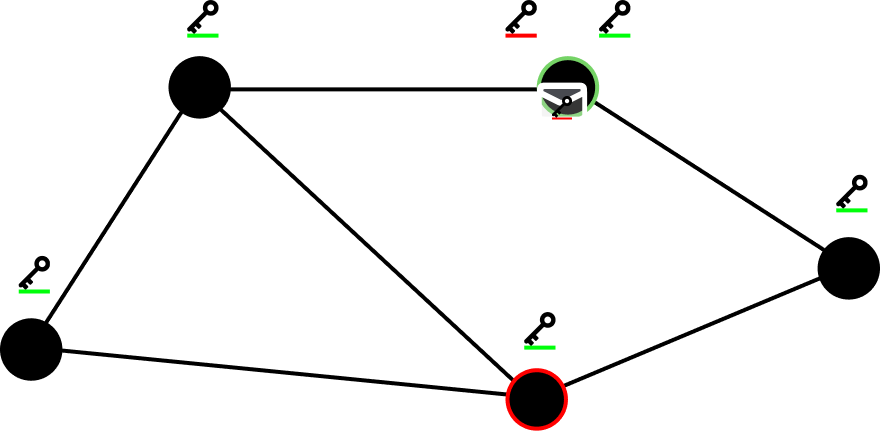
\includegraphics[width=0.7\textwidth]{Figures/Message sent.png}
    \caption{El nodo verde envía un mensaje.}
    \label{fg:messageSent}
\end{figure}
\begin{figure}[h!]
    \centering
    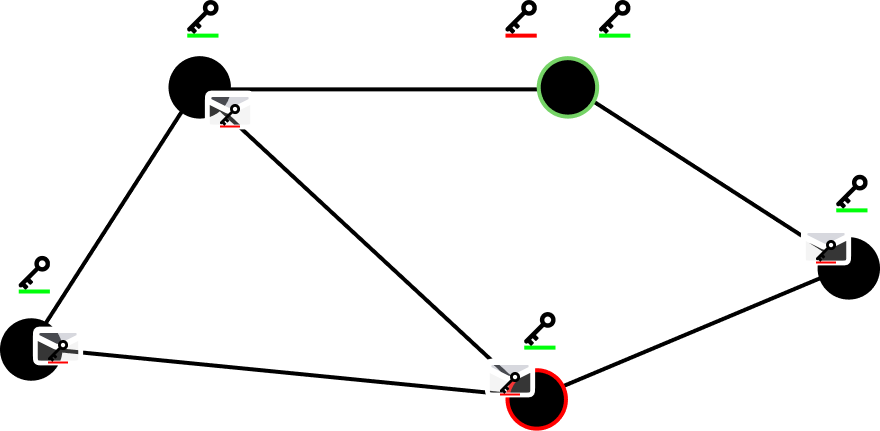
\includegraphics[width=0.7\textwidth]{Figures/Message arived.png}
    \caption{El resto de la red recibe el mensaje}
    \label{fg:messageRecived}
\end{figure}
Los mensajes salen del host verde firmados con su clave privada \ref{fg:messageSent}. Utilizando la clave publica del host verde (que han obtenido de la dirección original de IPFS \cite{web:ipfs}) pueden verificar la legitimidad del origen y actualizar su copia de la base de datos \ref{fg:messageRecived}.
\begin{figure}[h!]
    \centering
    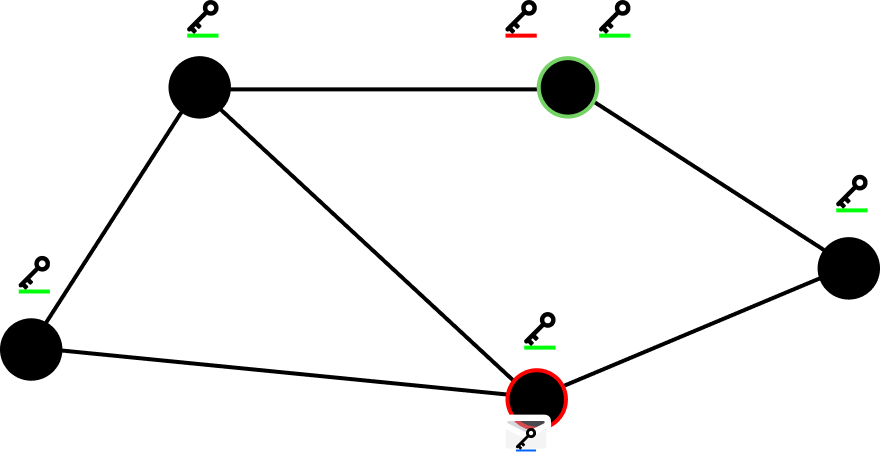
\includegraphics[width=0.7\textwidth]{Figures/Message is compromissed.png}
    \caption{El nodo rojo intenta sobrescribir la información de los nodos}
    \label{fg:messageSentRed}
\end{figure}
\begin{figure}[h!]
    \centering
    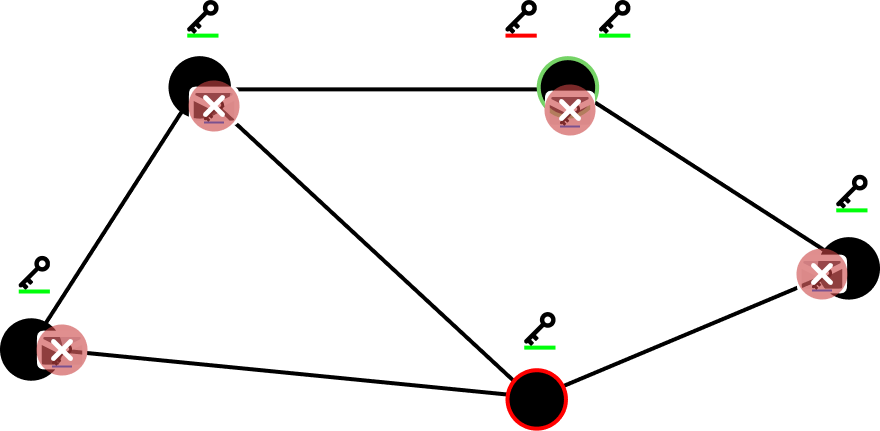
\includegraphics[width=0.7\textwidth]{Figures/Message rejected.png}
    \caption{El resto de la red }
\end{figure}
\newpage
\thispagestyle{empty}